\documentclass[border=3pt,tikz]{standalone}
\usepackage{amsmath}
\usetikzlibrary{arrows.meta}
\usetikzlibrary{calc}
\begin{document}
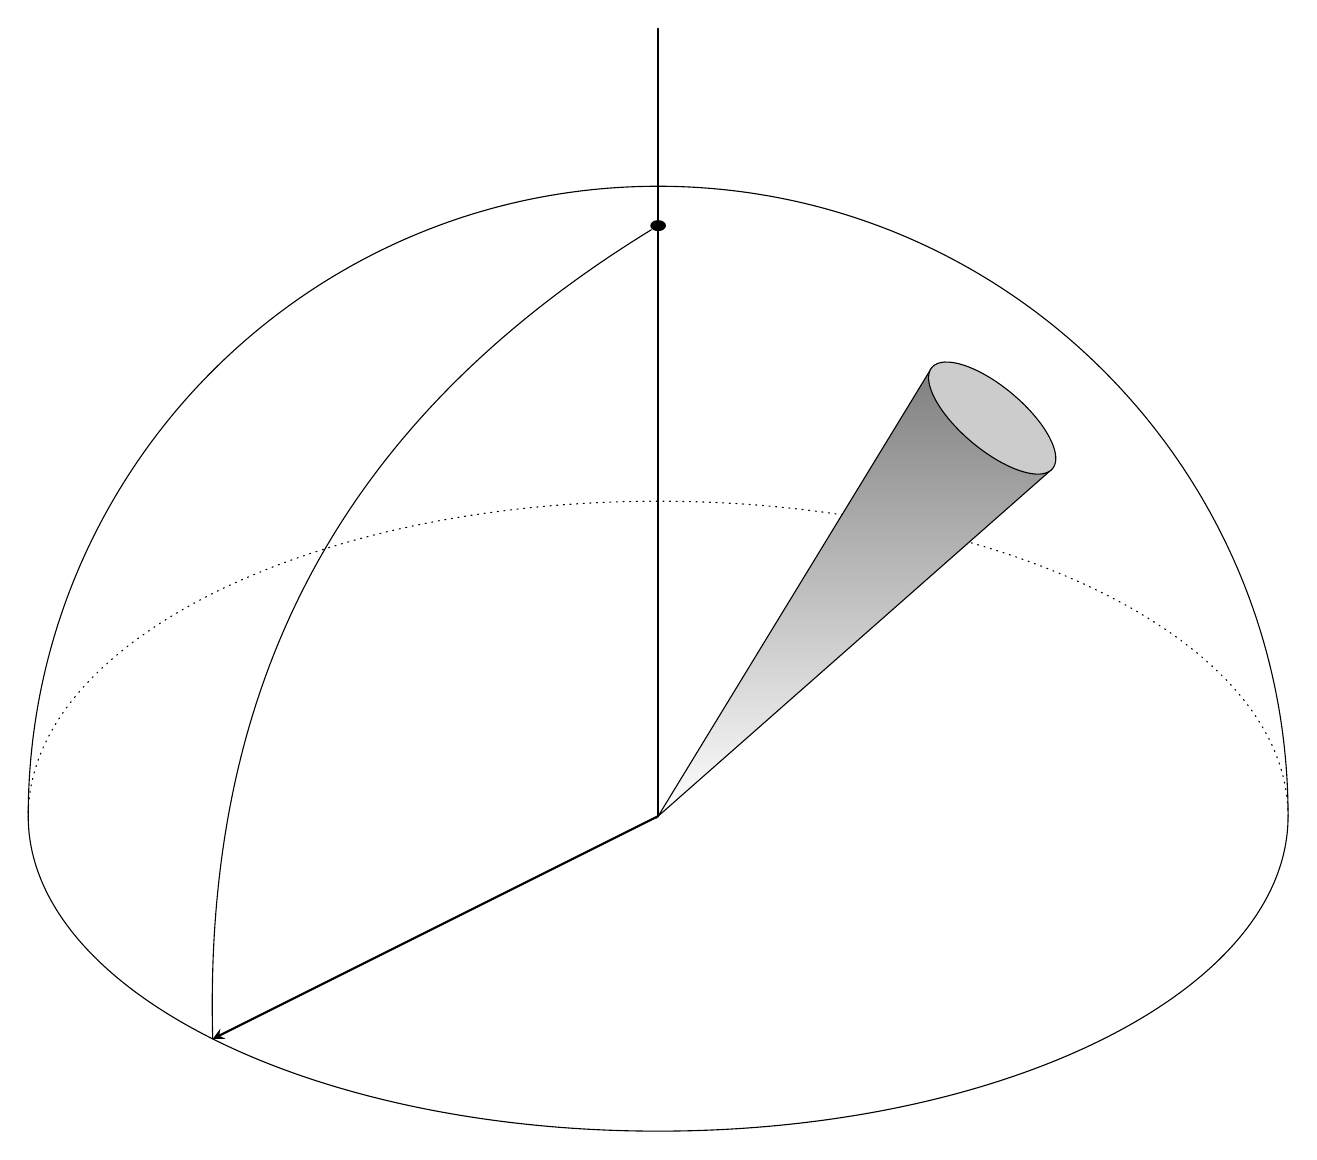
\begin{tikzpicture}[line cap=round, scale = 2]
    \draw (2,0) arc (-0:-180:4 and 2)coordinate[pos=0.75] (a);
    \draw[dotted] (2,0) arc (0:180:4 and 2);
    \draw (2,0) arc (0:180:4);
    \begin{scope}[rotate around={50:(-2,0)}]
    \draw[shade,fill=gray!40] (1.3, 0.5) -- (-2,0) -- (1.3,-0.5);
    \draw[fill=gray!40] (1.3,0) circle(0.2 and 0.5);
    \end{scope}
    \draw[thick,-stealth] (-2,0) -- (a);
    \draw[thick] (-2,0) -- node[pos=0.75,fill,inner sep=2pt,circle,yscale=0.7](b){}(-2,5);
    \draw (a) to[bend left] (b);
    \end{tikzpicture}
\end{document}